\section{Training an \ac{RNN} for \ac{ASR}}\label{ds}
As stated above, this project does not aim at training a state of the art \ac{STT} engine. Because the \ac{SW} algorithm used for local alignment is tolerant to a certain amount of errors in the transcripts, the \ac{RNN} need only be \textit{good enough} for the task at hand (\ac{FA}). If such a network can be trained under the given circumstances it could be used in the \ac{ASR} stage of the pipeline. The pipeline would then become become self-contained and would not ne dependent on a commercial solution that cannot eb tuned and whose inner workings are unknown. Furthermore such a \ac{RNN} would open up to recognizing languages for which there is not a third-party solution yet, such as Swiss German.

Hier etwas über Transfer Learning (z.B. wie in https://arxiv.org/pdf/1706.00290.pdf) und warum es nicht eingesetzt wurde (CNN anstatt RNN, Zeitaufwand). Layer Freezen bringt ausserdem offenbar auch nix. \parencite{budget}

\subsection{Exploiting the \textit{DeepSpeech} model}

A \ac{NN} that had quite an impact on \ac{ASR} was \textit{DeepSpeech} \parencite{deepspeech} which reached recognition rates near-par to human performance, despite using a comparably simpler than traditional speech systems. Because the relation between audio signal and text was learned \ac{E2E} the network was also pretty robust to distortions like background noise or speaker variation. An open source implementation of a DeepSpeech model is available from Mozilla \footnote{\url{https://github.com/mozilla/DeepSpeech}}. Since this implementation uses a \ac{LM}, the quality of the model is measured as the percentage of misspelled or wrong words (called \ac{WER}) or as the edit distance (also called Levenshtein distance or \ac{LER}). A pre-trained model for inference of English transcript can be downloaded, which achieves a \ac{WER} of just 6.5\%, which is close to what a human is able to recognize \parencite{mozillajourney}.

A model could be trained by providing training-, validation- and test-data for an arbitrary language (e.g. from the \textit{ReadyLingua} corpus). However, this is not the preferred procedure for this project for various reasons:

\begin{enumerate}
	\item The \textit{DeepSpeech} implementation was designed for \ac{ASR}. In such settings a low \ac{WER} is desirable. But this is not the main focus for this project. As a result, the architecture of the Mozilla implementation might be overly complicated for this project, although it might make sense for pure \ac{ASR} tasks. 
	\item The problem with above point is that more complex models usually require more training data. However, as for any neural network, the limiting factor for training a \ac{RNN} is often the lack of enough high quality training data. This becomes especially important when recordings in a minority language should be aligned. 
	\item The implementation requires an (optional) \ac{LM}, which is tightly integrated with the training process which might not be available for the target languages.
\end{enumerate}

For these reasons, the \ac{RNN} architecture of the \textit{DeepSpeech} model was used as a basis for a simplified version, which should (hopefully) require less training data in order to converge and still produce partial transcriptions that can be locally aligned.

\subsection{A simpler \textit{DeepSpeech} model}

An implementation of the \ac{RNN} used for \ac{STT} in the previous IP8 project was done in Python using Keras\footnote{\url{https://keras.io}}. This model is further referred to as \textit{previous model}. Unfortunately, this model did not perform well, i.e. it was not able to learn how to infer a transcript from a given sequence of feature vectors from a spectrogram.  Furthermore, performance was a big issue, although the \ac{RNN} used a simpler architecture and no computational power was needed to query a \ac{LM}. Training on aligned speech segments from the \textit{LibriSpeech} corpus was not possible within project time because it would have taken approximately two months when using a single ac{GPU}. This duration is at least consistent with the experience made by the Machine Learning team at Mozilla Research, which used a cluster of 16 \acsp{GPU} that required about a week \parencite{mozillajourney} to train a variant \footnote{the variant used \ac{MFCC} as features whereas the original paper proposed raw spectrograms} of the \ac{RNN} originally proposed in \parencite{ctc_paper}.

For this project, the previous model was closer examined to find out what works best and to help the model converge. After some changes to the previous model architecture for this project, a new model was obtained which was able to learn something meaningful, i.e. it started to infer transcripts that -- although still not perfect -- resembled the ground truth. This model is further referred to as \textit{new model}. Summarized, the following changes were made to the previous model architecture to constitute the new model:

\begin{itemize}
	\item \textbf{Optimizer}: The new model uses \ac{SGD} instead of Adam. Adam was used in the previous model because it was assumed to be generally superior to other other optimizers in most cases.
	\item \textbf{RNN cell type}: While \ac{LSTM} cells were used for the recurrent layer in the previous model, this was changed back to a simple RNN layer without gates as they appear in \ac{GRU} or \ac{LSTM} cells in the new model. This also corresponded to the original \textit{DeepSpeech} model architecture, which did not use sophisticated gated cells in their recurrent layer for computational reasons.
	\item \textbf{number of features}: While the use of \ac{MFCC} as features was examined in the previous model, the number of features was set to $13$, a value which is found often used in acoustic modelling. The Mozilla implementation of \textit{DeepSpeech} however doubled this number to $26$, which is also what is used in the new model. In spite of the increase in the number of features, this value is still much smaller than the $160$ filter banks used in the original \textit{DeepSpeech} model. The amount of training data is therefore still expected to be smaller than in the original model.
\end{itemize}

The final model used in this project was therefore a variant of the original \textit{DeepSpeech} model with the following simplifications:

\begin{itemize}
	\item \textbf{optional \ac{LM}}: While a key part in the original \textit{DeepSpeech} model, the inclusion of a  \ac{LM} is optional in the simplified architecture. This is on account of the fact that such a \ac{LM} needs to be trained first and to assess the influence of a trained \ac{LM} (see the following sections).
	\item No convolution in first layer
	\item LSTM instead of SimpleRNN
	\item \textbf{smaller alphabet}: The Mozilla implementation uses an alphabet of 29 characters (${a,b,c,...,z, space, apostrophe, blank}$), which is also what is proposed in the \textit{DeepSpeech} paper. This is due to the fact that apostrophes are frequently found in English word tokens (like \textit{"don't"} or \textit{"isn't"}). For simplification and also because a model should be trainable for any language, this character was dropped from the alphabet used in this project and also removed from the transcripts of all training samples by the normalization process. It is expected that missing apostrophes can be fixed by post-processing the inferred transcript with a \ac{LM}.
	\item \textbf{no context}: The \textit{DeepSpech} paper proposes using combining each feature vector $x_t$ (a frame in the spectrogram) with $C \in \left\{ 5,7,9 \right\}$ context frames. This context frame was dropped to keep the nuber of features in the input layer small. As a result, the first layer in the model only depends on the $26$ features of the feature vector $x_t$.
	\item \textbf{no convolution in input layer}: The \textit{DeepSpeech} paper proposes a series of optimization to reduce computational cost. Among these optimization is a convolution over time in the input layer with by striding with step size $2$. Because the context frame was dropped in this project, the striding was also not applied in order not to lose the information from the intermediate frames.
\end{itemize}


Figure \ref{model_architecture} shows the architecture proposed in the \textit{DeepSpeech} with the changes applied for this project. It looks similar to the one shown in the paper. Note the missing context frame, the use of \ac{MFCC} features and \ac{LSTM} cells in the recurrent layer.

\begin{figure}
	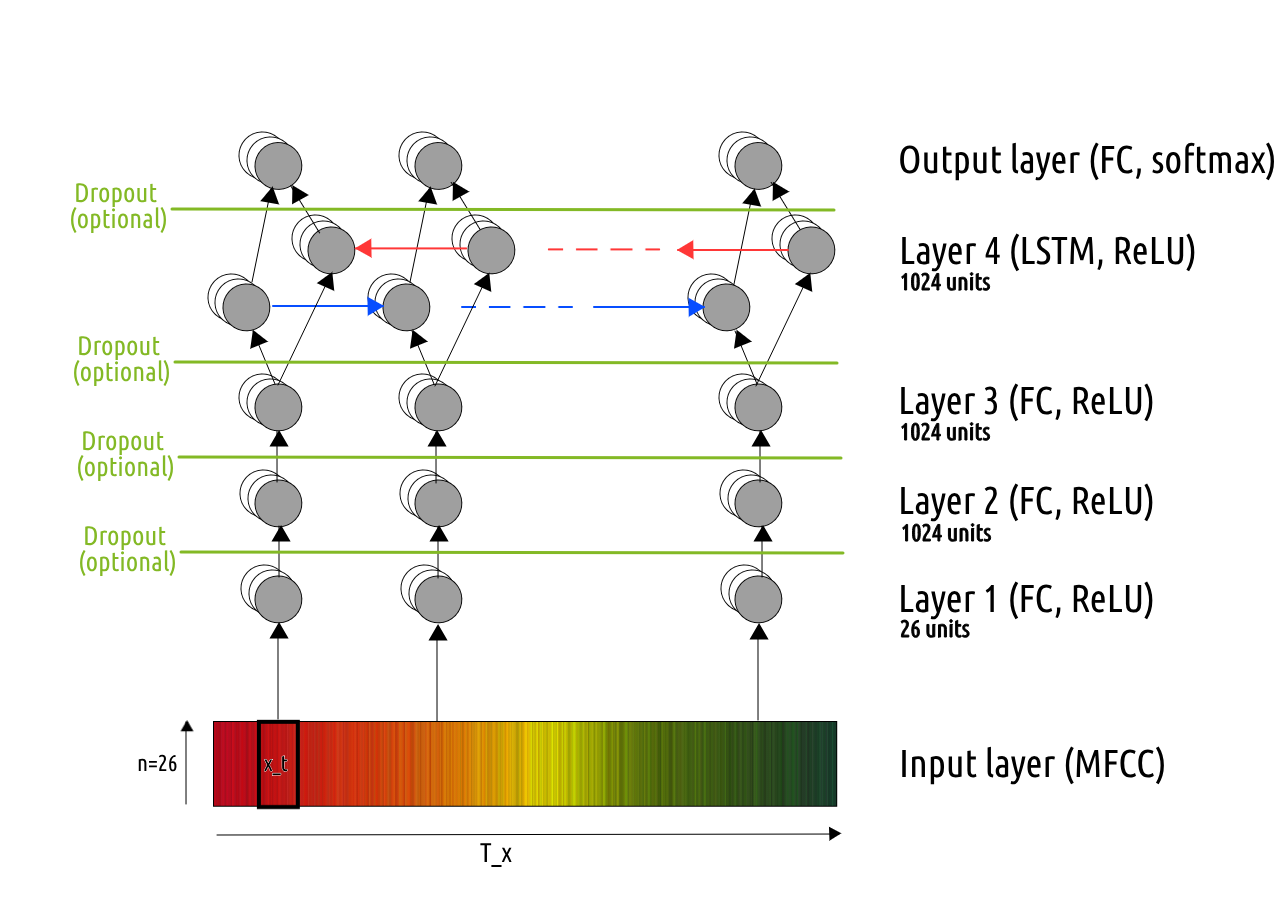
\includegraphics[width=\linewidth]{./img/model_architecture.png}
	\caption{architecture of the simplified model}
	\label{model_architecture}
\end{figure}


\section{The importance of \ac{LM}s for \ac{ASR}}

Although \ac{CTC} is the cost that is optimized during training, the usual metrics to evaluate an \ac{ASR} system are \ac{WER} and \ac{LER}. The \ac{LER} is defined as the mean normalized edit distance ($ed(a, b)$ i.e. the number of insertions, deletions and changes required to produce string $b$ from string $a$) between a an inferred transcription (\textit{prediction}) and the actual transcription (\textit{ground truth} or \textit{label}). It operates on character level and is sometimes also referred to as \textit{Levensthein Distance}. The \ac{WER} builds upon the \ac{LER} but operates on word level, i.e. it represents the number of words in a inferred transcription, that need to be inserted, deleted or changed in order to arrive at the ground truth.

If a single evaluation metric is required, the \ac{WER} is often the better choice because it is more related to the way humans would assess the quality of a transcription: A transcription which might sound correct when read out loud but is full of spelling mistakes is not a good transcription. A \ac{LM} can help inferring orthographically correct words from sequences of characters detected by \ac{CTC} and hence decrease the \ac{WER}. Therefore, by using a \ac{LM} the quality of transcriptions improves perceivably, as the following example shows:

\begin{table}[!htbp]
	\centering
	\begin{tabular}{|l|l|r|}
		\hline
		\thead{transcript} & \thead{value} & \thead{\ac{LER}} \\
		\hline
		actual transcript & \code{and i put the vice president in charge of mission control} & $1.00$ \\ 
		\hline
		inference without LM & \code{ii put he bice president in charge of mission control} & $0.11$ \\ 
		\hline
		inference with LM & \code{i put the vice president in charge of mission control} & $0.08$ \\
		\hline
	\end{tabular}
	\caption{examples of infered transcripts with pre-trained DeepSpeech model with and without \ac{LM}\\(sample \code{20161203potusweeklyaddress} from the ReadyLingua corpus}
\end{table}

A \ac{LM} models probabilities of sequences of words. Therefore a \ac{LM} can be used to assign a probability to a sentence. A simple \ac{LM} that does that is the $n$-gram \ac{LM}. $n$-grams are overlapping tuples of words whose probability can be approximated by training on massive text corpora. Although a lot of research has been made in the field of using \ac{NN} for language modelling (like for machine translation), $n$-grams \ac{LM} are still widely used and often the right tool for many tasks \parencite{slp3}, because they are faster to train and require significantly less training data.

The Mozilla implementation includes an $n$-Gram \ac{LM} using \textit{KenLM}. The \ac{LM} is queried while decoding the numeric matrices produced by \ac{CTC} using \textit{Beam Search} or \textit{Best-Path} decoding. It uses a \textit{trie} and precompiled custom implementations in C of \textit{TensorFlow}-operations to maximize performance and dedicated weights for the influence the number of valid words and the \ac{LM} itself on the inferred transcription. It is therefore deeply baked in with the decoding process.

A simpler variant that is used in this project is to infer the transcriptions first with \textit{Beam Search} or \textit{Best-Path} decoding using the standard tools provided by Keras. The inferred transcriptions are then post-processed by running it through some sort of spell-checking, which is done as follows:

\begin{itemize}
	\item split the sentence into words 
	\item for each word $w_i$ in the sentence check the spelling by generating the set $C_i$ of possible corrections by looking it up in $V$, the vocabulary of the \ac{LM}, as follows:
	\begin{itemize}
		\item if $w_i \in V$ its spelling is already correct and $w_i$ is kept as the only possible correction, i.e.
		\begin{equation*}
			C_i = C_j^0 = \{ w_i \}
		\end{equation*}
		\item if $w_i \not\in V$ generate $C_i^1$ as the set of all possible words $w_i^1$ with $ed(w_i, w_i^1) = 1$. This is the combined set of all possible words with one character inserted, deleted or replaced. Keep the words from this combined set that appear in $V$, i.e.
		\begin{equation*}
			C_i = C_i^1 = \left \{ w_i^1 \mid (w_i, w_i^1) = 1 \land w_i^1 \in V \right \}
		\end{equation*}
		\item if $C_i^1 = \emptyset$ generate $C_i^2$ as the set of all possible words $w_i^2$ with $ed(w_i, w_i^2) = 2$. $C_i^2$ can be recursively calculated from $C_i^1$. Again only keep the words that appear in $V$, i.e.
		\begin{equation*}
			C_i = C_i^2 = \left \{ w_i^2 \mid ed(w_i, w_i^2) = 2 \land w_i^2 \in V) \right \}
		\end{equation*}
		\item if $C_i^2 = \emptyset$ keep $w_i$ as the only word, accepting that it might be either misspelled, a wrong word, gibberish or simply has never been seen by the \ac{LM}, i.e.
		\begin{equation*}
			C_i = C_i{>2} = \left \{ w_i  \right \}
		\end{equation*}
	\end{itemize}
	\item for each possible spelling in $C_i$ build the set $P$ of all possible 2-grams with the possible spellings in the next word as the cartesian product of all words, i.e.
	\begin{flalign*}
&	P = \{ (w_j, w_{j+1} | w_j \in C_j \land w_{j+1} \in C_{j+1} \}{,} && C_j \in \{C_i^0, C_i^1, C_i^2, C_i^{>2} \}
	\end{flalign*}
	\item score each 2-gram calculating the log-based probability using a pre-trained 2-gram-\ac{LM}
\end{itemize}

\section{Plotting a learning curve}

The total length of all transcribed speech segments in the \textit{LibriSpeech} corpus is roughly 47 days (1,141 hours). Training on all these samples was not feasible within project time . However, we can get an estimation of the expected learning progress by plotting a \textit{learning curve}. This was done using transcribed audio segments from the \textit{LibriSpeech} corpus. Training was done on exponentially increasing amounts of training data (1, 10, 100 and 1000 minutes of transcribed audio). To assess the impact of using a \ac{LM}, the learning curve was plotted twice: Figure \ref{learning_curve_without_lm} shows the learning curve for \ac{WER} and \ac{LER} without using a \ac{LM}. Figure \ref{learning_curve_with_lm} shows the learning curve for training with a 4-gram \ac{LM}.

\begin{figure}
	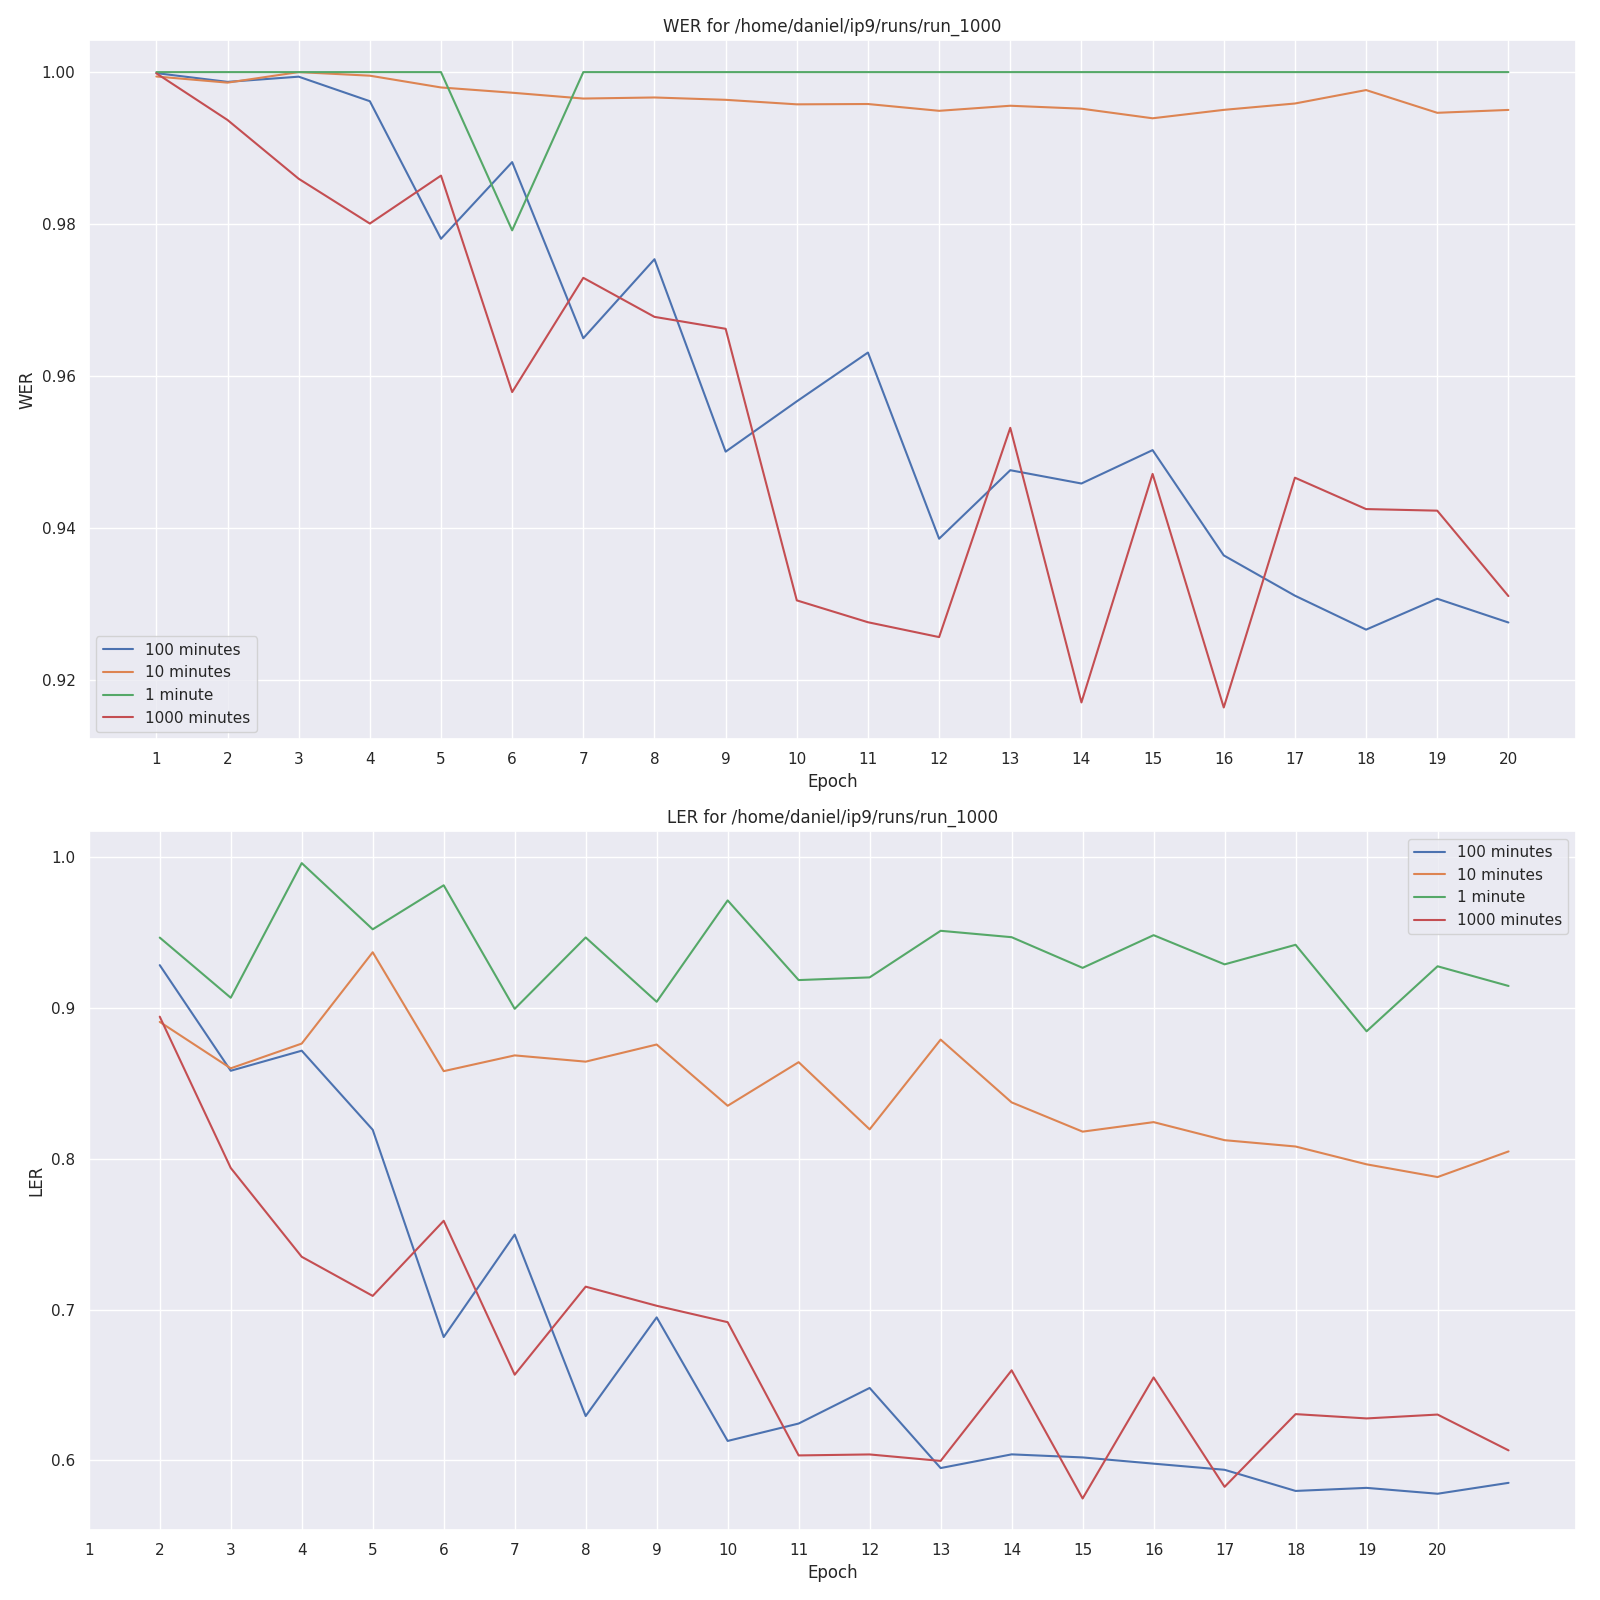
\includegraphics[width=\linewidth]{./img/learning_curve_lm_beamsearch.png}
	\caption{Learning curve for training on 1/10/100/1000 minutes of transcribed audio from \textit{ReadyLingua} using a 2-gram \ac{LM} and Beam-Search decoding}
	\label{learning_curve_without_lm}
\end{figure}

\begin{figure}
	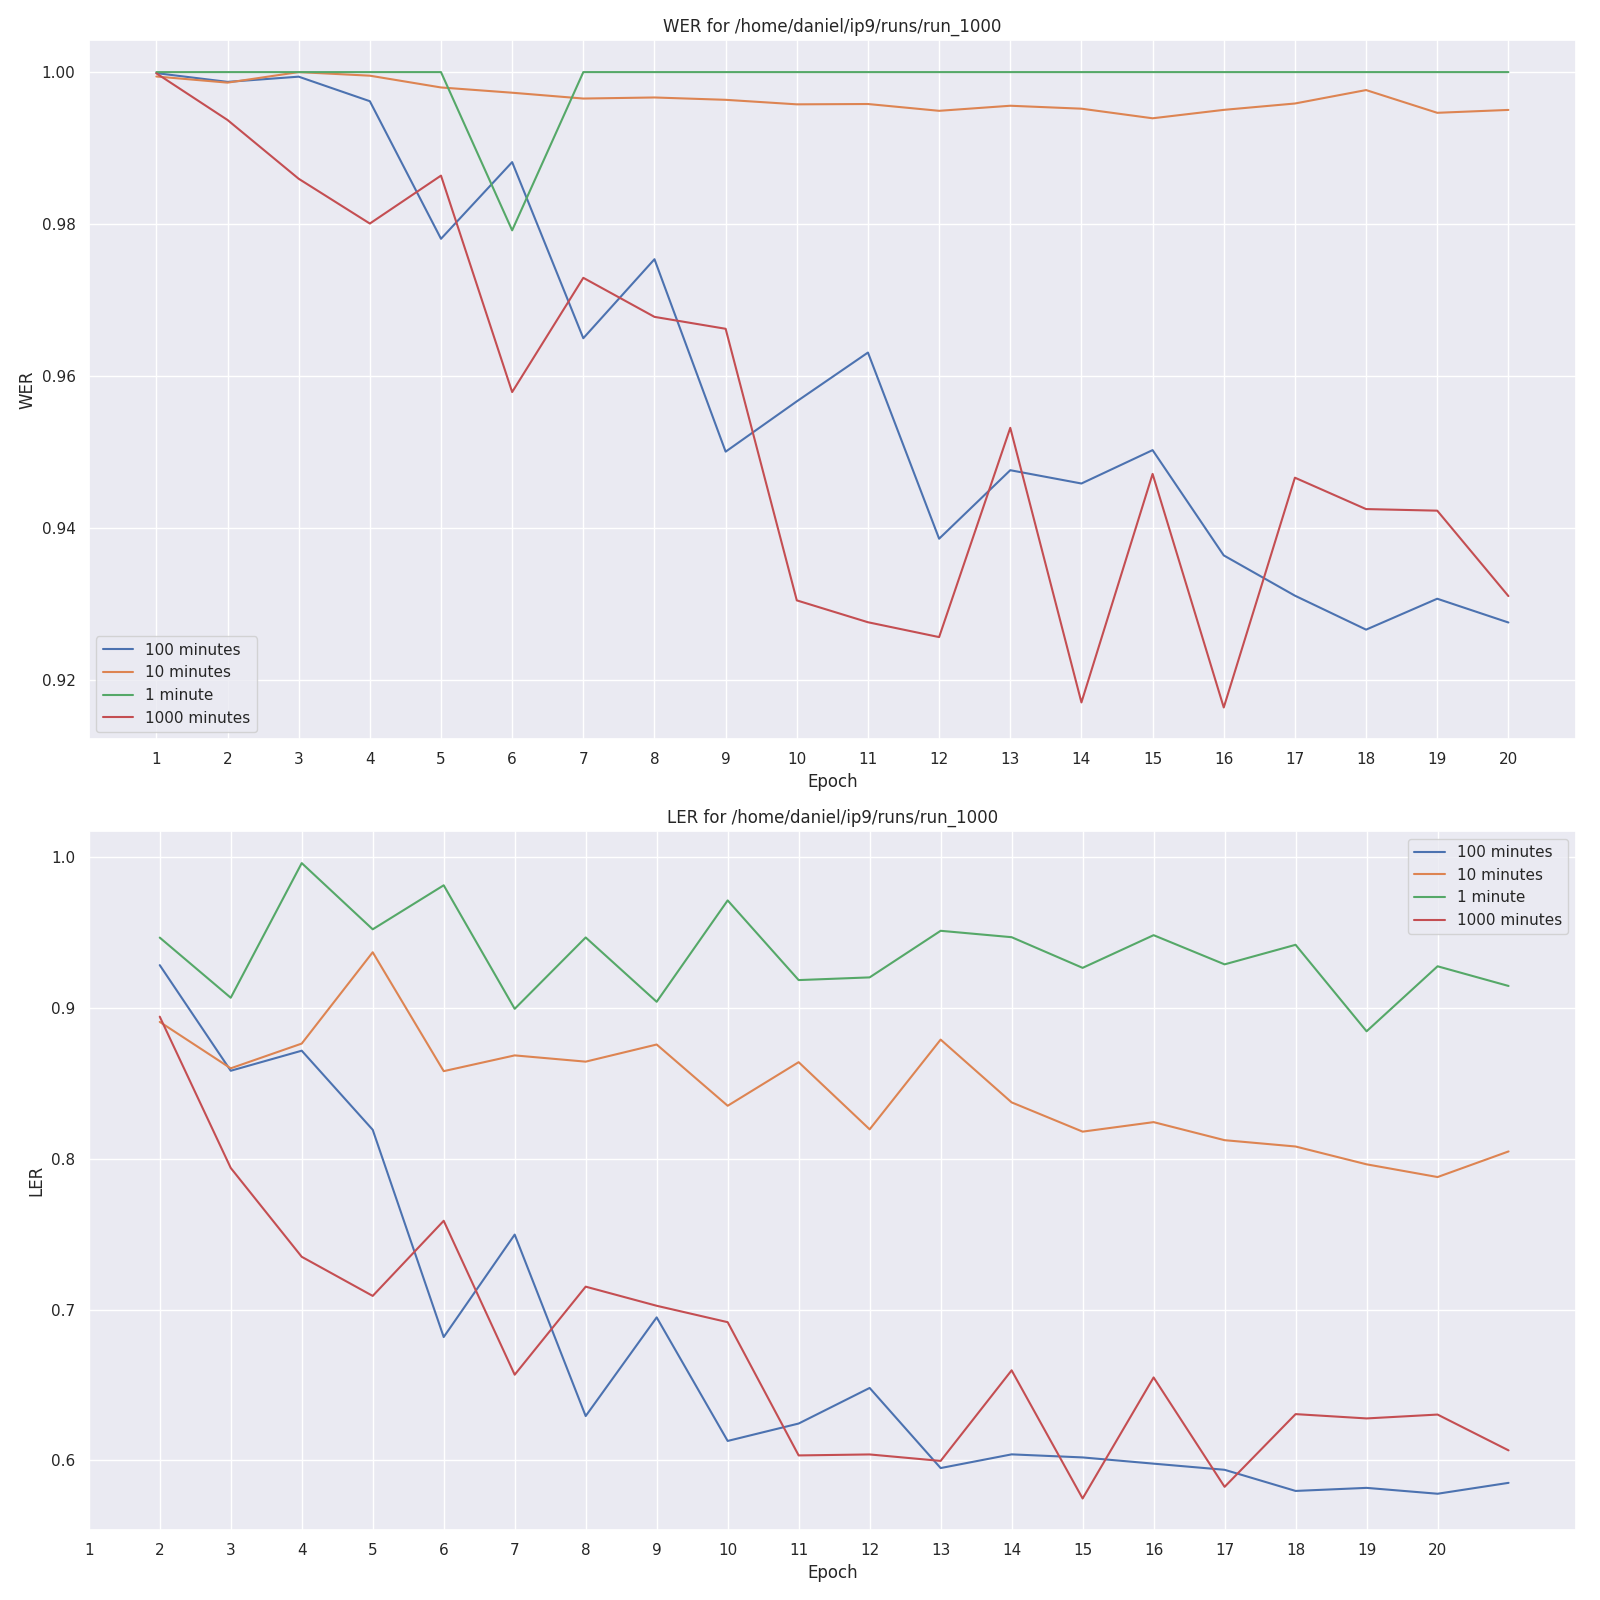
\includegraphics[width=\linewidth]{./img/learning_curve_lm_beamsearch.png}
	\caption{Learning curve for training on 1/10/100/1000 minutes of transcribed audio from \textit{ReadyLingua} using a 2-gram \ac{LM} and Beam-Search decoding}
	\label{learning_curve_with_lm}
\end{figure}

Hier etwas über

- Batchgrösse (Qualität nimmt mit zunehmender batchgrösse ab!)
- Padding der Trainingssequenzen
- Sortierung der Trainingsdaten nach Länge (ist besser, da weniger blanks gepadded)
- ...

% To do:
% - train on LibriSpeech data
% - train using Best-Path
% - train using no LM
% - Reset calculation of WER/LER to original implementation